%!TEX root = ../../report.tex
\chapter{Introduction}

Mobile robot navigation is highly based on offline generated maps of the environment. 
This is adequate in a lot of applications, but this approach can be insufficient in changing environments. 
As the discrepancy between the robot's internal map and the true state of the environment increases, tasks like path planning and localization will be based on increasingly erroneous data. 
To overcome these challenges, it would be beneficial to incorporate changes into the map.

As the environment changes, a robot which navigates by a predetermined static map will be prone to plan paths, that might have been blocked after the map was generated. 
If this happens, time would be wasted navigating around the obstacle.
The most simple solution to these problems would be adding or removing obstacles based on the latest observation. This, however, will likely clutter the map with highly dynamical obstacles, such as moving people or vehicles, thereby risk blocking large parts of the map. 
Therefore it is necessary to consider which obstacle should be included in the map, and how this selection is to be done.

\section{Aims}
This thesis aims to solve the problem of maintaining a consistent map of a dynamic environment over time. 
This is desired in order to improve localization and navigation of mobile robots. 
The focus of the project is on mapping the 2D ground level as this is widely used. 
The solution should be based on commonly used, on-board 2D LIDAR sensors, thus not requiring additional infrastructure to be established in the area of operation. 
It is chosen to make the solution easily integratable with common mobile robots, requiring no hardware changes. 
The platform used in this project is the MiR-100 \cite{mir-100-platform}.

In order to maintain an up-to-date representation of the world it is necessary to determine an effective way to represent dynamic and to continuously learn the dynamics of the environment. 
The learning must be able to account for changes in the dynamics, which occur in the environment over time. 
The method must be able to differentiate between static and dynamic obstacles.

 
As various sources of noise are expected in a real world scenario, these should be integrated into the learning system to provide a better basis for learning. One of the sources that should be considered is the LIDAR sensor noise, which could degrade the perception of the environment. 
Another is the localization noise.
As the system should run without extra infrastructure, the localization uncertainty in an on-board localization system should be taken into account.


In order to utilize the learned dynamics it is necessary to convert it into a usable map for the navigation and localization systems. Rules for this conversion will have to take into account the desired types of obstacles to represent. 
A user might want to only represent static obstacles, for instance walls and heavy machinery, for localization purposes but also more dynamic obstacles for navigation. 
As the exact classification parameters is dependent on the  application, it will most likely have to be adjusted for specific uses. 

Summing up, this project strives to improve navigation with mobile robots through continuous mapping of the operation area with on-board sensors. 
Specifically the following are considered:
\begin{enumerate}
    \item Precise mapping of static environments by incorporating sensor and localization noise
    \item Long-term, fast, adaptive map representation of dynamic environments
    \item Improved localization with a continuously adapted map of good features
    \item Integration and evaluation on the MiR-100 platform
\end{enumerate}

\section{Thesis core}
The system that has been devised in order to achieve the above mentioned goals can be considered in three main sections; static mapper, dynamic learner and cost interpretor. 
Figure \ref{fig:block-overview} shows an overview of the sections and their connections. 
The static mapper builds a occupancy grid map based on the sensor input received during a short time span. It is in this section the noise is handled by integrating a noise representation in the mapping method.
These short term maps are provided to the dynamics learner, which uses them to learn the dynamics of the world. The learner maintains a grid based representation of the dynamics. 
In order to provide a useful output for the navigation and localization systems the cost interpretor section handles the conversion from the dynamic representation. 

\begin{figure} [htbp]
	\centering
	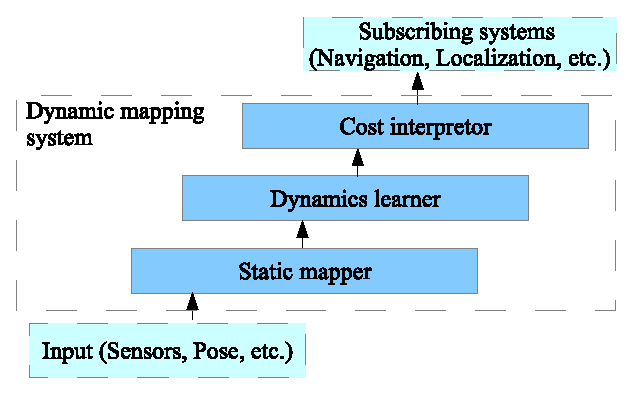
\includegraphics[scale=0.7]{chapters/introduction/figures/system-overview}
	\caption{Overview of the dynamic mapping system}
	\label{fig:block-overview}
\end{figure}

\subsection{Thesis outline}
First this thesis introduces the challenges in mapping dynamic areas. This is done with a focus on industrial environments and a short analysis is conducted to highlight the relevant characteristics.
Next the first of the static mapping is considered. 
This seeks to solve aim number 1. 
To do this various mapping methods and sensor models are evaluated.
Chapter \ref{mapping_of_dynamic_areas} investigates method for representing and learning the dynamics of an environment. 
Chapter \ref{chapter:cost_interpretation} describes the method used to generate output from the Static mapping system with respect to different uses. 
A short description of the architecture is also provided here. 
Lastly the the entire system is evaluated in chapter \ref{chapter:evaluation}.

The thesis is designed to follow the Dynamic mapping architecture from sensor input to output. 
In each chapter describing a section of the system an overview is provided to clarify the place of the section in the system. 
 
Appendix \ref{appendix:learning_curves} shows learning curves for the developed method.
Appendix \ref{appendix:pmac_pseudo_code} shows the pseudocode for a proposed learning method for Markov parameters.
Appendix \ref{appendix:usb_content} shows the content of the USB flash drive provided with the printed thesis. 

